% Gabarit pandoc des corrigés publiés (brut et guidé). Contenu sans marque ni nom de site.
% Compilation : lualatex (latexmk -lualatex).
% Le Markdown reste la source unique : ne pas éditer ce fichier .tex à la main.
\documentclass[11pt,a4paper]{article}

% --- Moteur, polices (Latin Modern) et langue ---------------------------------
\usepackage{iftex}
\ifLuaTeX\else\errmessage{Ce document se compile avec lualatex}\fi
\usepackage{amsmath,amssymb,mathtools}
\usepackage{fontspec}
% mathrm=sym : \mathrm prend ses glyphes dans la police mathématique (ℓ, μ, Ω), comme KaTeX.
\usepackage[math-style=TeX,bold-style=TeX,mathrm=sym]{unicode-math}
% Repli pour les glyphes absents de Latin Modern (indices et exposants Unicode,
% flèches, filets des schémas en texte, symboles) : DejaVu, puis Latin Modern Math
% (ℓ, lettres mathématiques Unicode des légendes).
\directlua{
  luaotfload.add_fallback("repliTexte", {"DejaVuSerif:mode=harf;", "DejaVuSans:mode=harf;", "file:latinmodern-math.otf:mode=harf;"})
  luaotfload.add_fallback("repliMono", {"DejaVuSansMono:mode=harf;", "DejaVuSans:mode=harf;", "file:latinmodern-math.otf:mode=harf;"})
}
\setmainfont{Latin Modern Roman}[RawFeature={fallback=repliTexte}]
\setsansfont{Latin Modern Sans}[RawFeature={fallback=repliTexte}]
\setmonofont{Latin Modern Mono}[RawFeature={fallback=repliMono}]
\setmathfont{Latin Modern Math}
\usepackage[french]{babel}
\frenchsetup{SmallCapsFigTabCaptions=false}

% --- Mise en page --------------------------------------------------------------
\usepackage[a4paper,margin=2.2cm,headheight=14pt,footskip=1.2cm]{geometry}
\usepackage{microtype}
\setlength{\emergencystretch}{4em}
\tolerance=1500
\setlength{\parindent}{0pt}
\setlength{\parskip}{0.55\baselineskip plus 2pt minus 1pt}
\usepackage{xcolor}
% Gris nommés : babel-french rend « ! » actif dans le document.
\definecolor{gris2}{gray}{0.98}
\definecolor{gris3}{gray}{0.97}
\definecolor{gris5}{gray}{0.95}
\definecolor{gris35}{gray}{0.65}
\definecolor{gris40}{gray}{0.60}
\definecolor{gris45}{gray}{0.55}
\definecolor{gris50}{gray}{0.50}
\definecolor{gris55}{gray}{0.45}
\definecolor{gris60}{gray}{0.40}
\definecolor{gris65}{gray}{0.35}
\definecolor{gris70}{gray}{0.30}
\definecolor{gris80}{gray}{0.20}
\definecolor{gris85}{gray}{0.15}
\usepackage{graphicx}
\usepackage{float}
\usepackage{caption}
\captionsetup{font=small,labelformat=empty,justification=centering}
\usepackage{booktabs,longtable,array,multirow,calc}
\usepackage{siunitx}
\sisetup{locale=FR}
\usepackage[version=4]{mhchem}
\usepackage{listings}
\usepackage{fancyhdr}
\usepackage{lastpage}
\usepackage[most]{tcolorbox}
\usepackage{enumitem}
\setlist{nosep,leftmargin=*,topsep=2pt}
\usepackage[hidelinks,unicode]{hyperref}
\usepackage{bookmark}
\hypersetup{pdftitle={CCINP TPC — Physique 2026},pdfauthor={Rédigé par IA},pdfcreator={LaTeX},pdfsubject={Corrigé brut}}
\usepackage{xurl}

% --- Pandoc : listes, tableaux, figures ----------------------------------------
\providecommand{\passthrough}[1]{#1}
\providecommand{\tightlist}{\setlength{\itemsep}{0pt}\setlength{\parskip}{0pt}}

\makeatletter
\def\maxwidth{\ifdim\Gin@nat@width>\linewidth\linewidth\else\Gin@nat@width\fi}
\def\maxheight{\ifdim\Gin@nat@height>0.55\textheight 0.55\textheight\else\Gin@nat@height\fi}
\makeatother
\setkeys{Gin}{width=\maxwidth,height=\maxheight,keepaspectratio}
\setcounter{secnumdepth}{-\maxdimen}
\providecommand{\pandocbounded}[1]{#1}
\usepackage{longtable,booktabs,array}

% --- Code (listings) -----------------------------------------------------------
\lstset{
  basicstyle=\ttfamily\small,
  columns=fullflexible,
  keepspaces=true,
  breaklines=true,
  breakatwhitespace=false,
  postbreak=\mbox{\textcolor{gris50}{$\hookrightarrow$}\space},
  frame=single,
  rulecolor=\color{gris35},
  framesep=4pt,
  xleftmargin=5pt,xrightmargin=5pt,
  backgroundcolor=\color{gris3},
  keywordstyle=\bfseries,
  commentstyle=\color{gris65},
  stringstyle=\color{gris80},
  showstringspaces=false,
  tabsize=4,
  extendedchars=true,
  aboveskip=6pt,belowskip=6pt,
}

% --- Macros des corrigés (KaTeX ↔ LaTeX) ---------------------------------------
% Les corrigés sont écrits pour KaTeX : on définit ici ce que KaTeX connaît et
% que LaTeX n'a pas, sans jamais retoucher le Markdown.
\providecommand{\R}{\mathbb{R}}
\providecommand{\N}{\mathbb{N}}
\providecommand{\Z}{\mathbb{Z}}
\providecommand{\Q}{\mathbb{Q}}
\providecommand{\C}{\mathbb{C}}
\providecommand{\dd}{\mathrm{d}}
\providecommand{\llbracket}{\lBrack}
\providecommand{\rrbracket}{\rBrack}
\providecommand{\lBrace}{\lbrace}
\providecommand{\rBrace}{\rbrace}
\providecommand{\Box}{\square}
\providecommand{\Diamond}{\lozenge}
\providecommand{\varnothing}{\emptyset}
\providecommand{\argmax}{\operatorname*{arg\,max}}
\providecommand{\argmin}{\operatorname*{arg\,min}}
\renewcommand{\leq}{\leqslant}
\renewcommand{\geq}{\geqslant}

% Équation hors texte : réduite à la largeur de la ligne si elle déborde.
\newsavebox{\boiteequation}
\newcommand{\equationajustee}[1]{%
  \sbox{\boiteequation}{$\displaystyle #1$}%
  \ifdim\wd\boiteequation>\linewidth
    \[\resizebox{\linewidth}{!}{\usebox{\boiteequation}}\]%
  \else
    \[#1\]%
  \fi}

% --- Encadrés pédagogiques (sobres, lisibles en noir et blanc) -----------------
\tcbset{
  encadre/.style={
    enhanced,breakable,sharp corners,
    colback=white,colframe=gris55,
    boxrule=0.4pt,leftrule=2.2pt,
    left=6pt,right=6pt,top=3pt,bottom=3pt,
    before skip=6pt,after skip=6pt,
    fonttitle=\bfseries\small,coltitle=black,
    attach title to upper,after title={\quad},
    parbox=false,
  }
}
\newtcolorbox{indication}[1]{encadre,colframe=gris45,colback=gris2,title={Indication~#1}}
\newtcolorbox{methode}{encadre,colframe=gris70,title={Méthode}}
\newtcolorbox{piege}{encadre,colframe=gris85,boxrule=0.8pt,leftrule=2.2pt,title={Piège}}
\newtcolorbox{jury}{encadre,colframe=gris60,colback=gris5,title={Jury}}
\newtcolorbox{encadrenote}{encadre,colframe=gris40}

% --- Titres de section ---------------------------------------------------------
\usepackage{titlesec}
\titleformat{\section}{\Large\bfseries}{}{0pt}{}
\titleformat{\subsection}{\large\bfseries}{}{0pt}{}
\titleformat{\subsubsection}{\normalsize\bfseries}{}{0pt}{}
\titlespacing*{\section}{0pt}{14pt plus 4pt minus 2pt}{6pt}
\titlespacing*{\subsection}{0pt}{10pt plus 3pt minus 2pt}{4pt}
\titlespacing*{\subsubsection}{0pt}{8pt plus 2pt minus 2pt}{2pt}

% --- En-tête et pied de page ---------------------------------------------------
\pagestyle{fancy}
\fancyhf{}
\fancyhead[L]{\small\textsc{Corrigé brut} · CCINP TPC}
\fancyhead[R]{\small Physique 2026}
\fancyfoot[L]{\footnotesize Corrigé rédigé par IA, non officiel}
\fancyfoot[R]{\footnotesize \thepage\,/\,\pageref*{LastPage}}
\renewcommand{\headrulewidth}{0.4pt}
\renewcommand{\footrulewidth}{0pt}
\fancypagestyle{plain}{\fancyhf{}\fancyfoot[R]{\footnotesize \thepage\,/\,\pageref*{LastPage}}\fancyfoot[L]{\footnotesize Corrigé rédigé par IA, non officiel}\renewcommand{\headrulewidth}{0pt}}

\begin{document}
\thispagestyle{plain}
\begin{center}
  {\small\scshape Corrigé brut}\par\smallskip
  {\LARGE\bfseries CCINP TPC — Physique 2026\par}\medskip
  {\large CCINP · TPC · Physique · 2026\par}
\end{center}
\vspace{2pt}\hrule\vspace{8pt}

\emph{Corrigé rédigé par IA, non officiel. Signalez toute erreur.}

Épreuve TPC2P, 4 heures, calculatrices interdites. Deux problèmes indépendants.

Problème I --- Physique du pop-corn

\hypertarget{partie-i-diffusion-thermique-dans-un-grain-de-mauxefs}{%
\section{Partie I --- Diffusion thermique dans un grain de maïs}\label{partie-i-diffusion-thermique-dans-un-grain-de-mauxefs}}

\hypertarget{q1}{%
\subsection{Q1}\label{q1}}

\equationajustee{\begin{aligned}
{[\lambda]}&=\mathrm{W\cdot K^{-1}\cdot m^{-1}}\\
&=\mathrm{J\cdot s^{-1}\cdot K^{-1}\cdot m^{-1}}\\
{[\rho c]}&=\mathrm{kg\cdot m^{-3}}\times\mathrm{J\cdot K^{-1}\cdot kg^{-1}}\\
&=\mathrm{J\cdot K^{-1}\cdot m^{-3}}
\end{aligned}}
Le quotient vaut
\equationajustee{\boxed{[D_{th}]=\mathrm{m^2\cdot s^{-1}}}}

\hypertarget{q2}{%
\subsection{Q2}\label{q2}}

La durée cherchée ne dépend que de la taille \(a\) et de la diffusivité \(D_{th}\), seul coefficient de transport du problème (loi d'échelle de la diffusion construite par analyse dimensionnelle). On cherche \(\tau_{diff}=a^\alpha D_{th}^\beta\) :
\equationajustee{\begin{aligned}
\mathrm{T}&={\mathrm{L}}^{\alpha}\left({\mathrm{L}}^2{\mathrm{T}}^{-1}\right)^{\beta}\\
&={\mathrm{L}}^{\alpha+2\beta}\,{\mathrm{T}}^{-\beta}
\end{aligned}}
On identifie les exposants du temps et de la longueur :
\equationajustee{\begin{aligned}
-\beta&=1\\
\alpha+2\beta&=0
\end{aligned}}
d'où \(\beta=-1\) et \(\alpha=2\).
À un facteur numérique sans dimension près, pris égal à 1 :
\equationajustee{\boxed{\tau_{diff}=\frac{a^2}{D_{th}}}}

\hypertarget{q3}{%
\subsection{Q3}\label{q3}}

\equationajustee{\begin{aligned}
D_{th}&=\frac{0{,}2}{1\cdot10^3\times2\cdot10^3}\\
&=1\cdot10^{-7}\ \mathrm{m^2\cdot s^{-1}}
\end{aligned}}
puis
\equationajustee{\begin{aligned}
\tau_{diff}&=\frac{(3\cdot10^{-3})^2}{1\cdot10^{-7}}\\
&=\frac{9\cdot10^{-6}}{1\cdot10^{-7}}
\end{aligned}}
\equationajustee{\boxed{\tau_{diff}\simeq9\cdot10^1\ \mathrm{s}}}
C'est la durée donnée pour le germe dans le tableau 1. Le temps de cuisson (de l'ordre de la minute) est du même ordre que \(\tau_{diff}\), et non très grand devant lui : \textbf{le régime de diffusion dans le grain entier ne peut pas être considéré comme permanent} pendant la cuisson.

\hypertarget{q4}{%
\subsection{Q4}\label{q4}}

Pour l'enveloppe, \(\tau_{env}=0{,}1\) s. Les conditions aux limites qu'elle subit (température de surface, température de l'amande vitreuse) évoluent sur les durées des zones internes (7 s à 90 s) et sur la durée de cuisson (\(\sim60\) s) :
\equationajustee{\frac{\tau_{env}}{t_{cuisson}}\sim\frac{0{,}1}{60}\sim2\cdot10^{-3}\ll1 .}
Le profil de température dans l'enveloppe s'adapte quasi instantanément à ces conditions : à chaque instant, il est celui du régime stationnaire correspondant aux températures de bord de cet instant. \textbf{La diffusion dans l'enveloppe est quasi stationnaire.}

\hypertarget{q5}{%
\subsection{Q5}\label{q5}}

La calotte (deux sphères concentriques, matériau homogène, bain isotrope) est invariante par toute rotation autour du centre \(O\). Le champ scalaire \(T\) a les mêmes invariances : \(T\) ne dépend ni de \(\theta\) ni de \(\varphi\), \(T=T(r)\) (le temps n'intervenant que comme paramètre en régime quasi stationnaire). Le gradient en sphériques se réduit à son terme radial et la loi de Fourier donne
\equationajustee{\boxed{\vec j_{th}=-\lambda\frac{\mathrm dT}{\mathrm dr}\,\vec e_r=j_{th}(r)\,\vec e_r}}
L'huile (200 °C) est plus chaude que le grain : la chaleur va de l'extérieur vers le centre, selon \(-\vec e_r\). Donc \(\boxed{j_{th}(r)<0}\).

\hypertarget{q6}{%
\subsection{Q6}\label{q6}}

On compte \(\Phi_{th}(r)\) positivement vers le centre : \(\Phi_{th}(r)=-4\pi r^2j_{th}(r)>0\). Premier principe pour la coquille comprise entre \(r\) et \(r+\mathrm dr\) (système fermé, pas de travail, pas de source interne), de capacité thermique \(\mathrm dC\), pendant \(\mathrm dt\) :
\equationajustee{\mathrm dC\,\frac{\partial T}{\partial t}=\Phi_{th}(r+\mathrm dr)-\Phi_{th}(r) .}
En régime quasi stationnaire (Q4), le membre de gauche est négligeable, d'où \(\Phi_{th}(r+\mathrm dr)=\Phi_{th}(r)\) :
\equationajustee{\boxed{\frac{\mathrm d\Phi_{th}}{\mathrm dr}=0\ :\ \Phi_{th}\ \text{est \text{indépendant} de}\ r}}

\hypertarget{q7}{%
\subsection{Q7}\label{q7}}

D'après Q6, \(j_{th}(r)=-\dfrac{\Phi_{th}}{4\pi r^2}\) ; d'après Q5, \(j_{th}=-\lambda\dfrac{\mathrm dT}{\mathrm dr}\). Donc
\equationajustee{\frac{\mathrm dT}{\mathrm dr}=\frac{\Phi_{th}}{4\pi\lambda r^2}}
Une primitive de \(1/r^2\) étant \(-1/r\) :
\equationajustee{\boxed{T(r)=-\frac{\Phi_{th}}{4\pi\lambda}\,\frac1r+K}}
Contrôle : \(\mathrm dT/\mathrm dr>0\), la température croît vers l'extérieur, ce qui est la situation physique.

\hypertarget{q8}{%
\subsection{Q8}\label{q8}}

La résistance thermique est définie par \(\Delta T=R_{th}\Phi_{th}\), avec \(\Delta T=T(R_2)-T(R_1)\) :
\equationajustee{\boxed{R_{th}=\frac{T(R_2)-T(R_1)}{\Phi_{th}}}}
Elle s'exprime en \(\mathrm{K\cdot W^{-1}}\).

\begin{longtable}[]{@{}
  >{\raggedright\arraybackslash}p{(\columnwidth - 2\tabcolsep) * \real{0.5000}}
  >{\raggedright\arraybackslash}p{(\columnwidth - 2\tabcolsep) * \real{0.5000}}@{}}
\toprule\noalign{}
\begin{minipage}[b]{\linewidth}\raggedright
Grandeur thermique
\end{minipage} & \begin{minipage}[b]{\linewidth}\raggedright
Équivalent électrocinétique
\end{minipage} \\
\midrule\noalign{}
\endhead
\bottomrule\noalign{}
\endlastfoot
écart de température \(\Delta T\) (K) & tension \(U\) (V) \\
flux thermique \(\Phi_{th}\) (W) & intensité \(I\) (A) \\
résistance thermique \(R_{th}\) (K·W⁻¹) & résistance électrique \(R\) (Ω) \\
\end{longtable}

La relation \(\Delta T=R_{th}\Phi_{th}\) est l'analogue de la loi d'Ohm \(U=RI\).

\hypertarget{q9}{%
\subsection{Q9}\label{q9}}

Avec Q7 :
\equationajustee{\begin{aligned}
\Delta T&=-\frac{\Phi_{th}}{4\pi\lambda}\left(\frac1{R_2}-\frac1{R_1}\right)\\
&=\frac{\Phi_{th}}{4\pi\lambda}\,\frac{R_2-R_1}{R_1R_2}
\end{aligned}}
d'où
\equationajustee{\boxed{R_{th}=\frac{R_2-R_1}{4\pi\lambda R_1R_2}}}
Le tableau 1 donne l'épaisseur de l'enveloppe \(e=R_2-R_1=0{,}1\) mm pour \(R_2=a=3\) mm : \(e/a\simeq3\cdot10^{-2}\ll1\), donc \(R_1R_2\simeq a^2\) et
\equationajustee{\boxed{R_{th}\simeq\frac{e}{\lambda S}}}
avec
\equationajustee{e=R_2-R_1}
\equationajustee{S=4\pi R_1R_2\simeq4\pi a^2}
\textbf{Commentaire} : l'enveloppe étant très mince devant le rayon, sa courbure est négligeable ; on retrouve la résistance d'un mur plan d'épaisseur \(e\) et de section égale à la surface du grain. À titre indicatif, \(S\simeq1{,}1\cdot10^{-4}\) m² et \(R_{th}\simeq4\) K·W⁻¹.

\hypertarget{q10}{%
\subsection{Q10}\label{q10}}

La loi de Newton s'écrit \(T_{ext}-T_S=\Phi_{th}/(hS_S)\) ; par identification avec \(\Delta T=R\,\Phi_{th}\) :
\equationajustee{\boxed{R_{cc}=\frac1{h\,S_S}}}

\hypertarget{q11}{%
\subsection{Q11}\label{q11}}

Le même flux \(\Phi_{th}\) traverse l'interface huile-grain puis l'enveloppe (pas d'accumulation, Q6), et les écarts de température s'ajoutent :
\equationajustee{T_{ext}-T(R_1)=(T_{ext}-T_S)+(T_S-T(R_1))=(R_{cc}+R_{th})\,\Phi_{th} .}
Les deux résistances sont \textbf{en série}. Avec \(S\simeq S_S\) (enveloppe mince) :
\equationajustee{\boxed{R_{eq}=R_{cc}+R_{th}\simeq\frac1{S_S}\left(\frac1h+\frac e\lambda\right)}}

\begin{figure}[H]
\centering
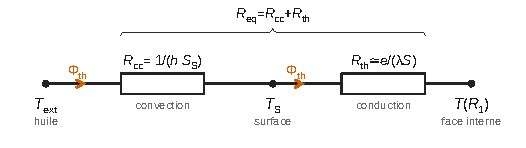
\includegraphics{figures/q11-resistances-serie.pdf}
\caption*{Figure 1 --- Schéma électrique équivalent, les résistances
conducto-convective et de l'enveloppe traversées par le même flux sont
en série}
\end{figure}

\hypertarget{q12}{%
\subsection{Q12}\label{q12}}

Le flux reçu par l'intérieur du grain vaut \(\Phi_{th}=(T_{ext}-T(R_1))/R_{eq}\), avec \(R_{eq}\simeq\dfrac1{S_S}\left(\dfrac1h+\dfrac e\lambda\right)\). Or l'épaisseur \(e\) de l'enveloppe, la surface \(S_S\) et l'état de surface (qui influe sur \(h\)) varient d'un grain à l'autre (grandeurs biologiques dispersées ; l'énoncé ne donne que des valeurs moyennes). \(R_{eq}\), donc le flux reçu et la vitesse de montée en température de l'amande farineuse, varient d'un grain à l'autre : le seuil d'éclatement est atteint à des dates différentes. De plus, la résistance mécanique de l'enveloppe, qui dépend de son épaisseur, fixe la pression de rupture et varie elle aussi.
\equationajustee{\boxed{e\ (\text{et}\ S_S)\ \text{variant d'un grain \text{à} l'autre,}\ R_{eq}\ \text{et la date d'\text{éclatement} varient}}}

\hypertarget{partie-ii-uxe9clatement-et-saut-du-grain-de-mauxefs}{%
\section{Partie II --- Éclatement et saut du grain de maïs}\label{partie-ii-uxe9clatement-et-saut-du-grain-de-mauxefs}}

\hypertarget{q13}{%
\subsection{Q13}\label{q13}}

Figure 4 : \(P_{sat}=9\) bar pour \(T_r\simeq175\) °C. Figure 5 : l'eau se trouve dans l'amande farineuse, dont la courbe atteint 175 °C vers
\equationajustee{\boxed{t_{\text{\text{éclatement}}}\simeq1{,}3\cdot10^2\ \mathrm s\simeq2\ \text{min}}}
\textbf{Commentaire} : c'est l'ordre de grandeur observé pour la cuisson du pop-corn (une à deux minutes) et environ \(3\,\tau_{diff}\) de l'amande farineuse (45 s). La courbe approche son plafond (vers 183 °C) : la date est très sensible au seuil lu ; un seuil de 178 °C repousserait l'éclatement vers 140 s.

\hypertarget{q14}{%
\subsection{Q14}\label{q14}}

À \(t\simeq125\) s, l'enveloppe (≈195 °C) et l'amande vitreuse (≈190 °C) sont sur leur plateau ; l'amande farineuse (≈175 °C) et surtout le germe (≈138 °C) voient encore leur température croître nettement. \textbf{Non, le régime permanent n'est pas établi dans toutes les zones} : il ne l'est pas dans l'amande farineuse ni dans le germe.

Pour une zone, la montée est de type premier ordre, \(T(t)=T_\infty-(T_\infty-T_0)\,\mathrm e^{-t/\tau}\), où \(\tau\sim\ell^2/D_{th}\) ne dépend pas de la température de l'huile, et \(T_\infty\) croît avec \(T_{ext}\). Le seuil \(T_r\) est franchi à
\equationajustee{t_r=\tau\ln\frac{T_\infty-T_0}{T_\infty-T_r}}
Sa dérivée par rapport à \(T_\infty\) est négative, puisque \(T_\infty-T_r<T_\infty-T_0\) :
\equationajustee{\frac{\mathrm dt_r}{\mathrm dT_\infty}=\tau\left(\frac1{T_\infty-T_0}-\frac1{T_\infty-T_r}\right)<0 .}
\textbf{Oui, augmenter la température de l'huile raccourcit la durée nécessaire à l'éclatement} (dans la limite où le grain ne brûle pas et l'huile ne se dégrade pas).

\hypertarget{q15}{%
\subsection{Q15}\label{q15}}

\equationajustee{\begin{aligned}
n&=\frac{P_rV_0}{RT_r}\\
&=\frac{9\cdot10^5\times1\cdot10^{-7}}{4\cdot10^3}\\
&=2{,}25\cdot10^{-5}\ \mathrm{mol}
\end{aligned}}
puis
\equationajustee{\begin{aligned}
m_{vap}&=nM\\
&=2{,}25\cdot10^{-5}\times18\cdot10^{-3}
\end{aligned}}
\equationajustee{\boxed{m_{vap}\simeq4\cdot10^{-7}\ \mathrm{kg}=0{,}4\ \mathrm{mg}}}
Le grain contient \(0{,}10\times100=10\) mg d'eau : seuls 4 \% de l'eau sont sous forme vapeur juste avant l'éclatement. L'essentiel reste liquide, ce qui justifie l'équilibre liquide-vapeur (\(P=P_{sat}(T)\)) et fournit une réserve d'eau qui se vaporise lors de la détente.

\hypertarget{q16}{%
\subsection{Q16}\label{q16}}

Système fermé \(\{\)vapeur d'eau\(\}\), \(n\) fixé (la vapeur ne s'échappe pas). La détente réelle est brutale, donc irréversible, et ni la pression extérieure ni \(\gamma\) ne sont fournis. On l'estime par le modèle isotherme réversible à \(T_r\) (la vapeur reste au contact de l'eau liquide et de l'amidon) : \(P=nRT_r/V\) et
\equationajustee{\begin{aligned}
W&=-\int_{V_0}^{5V_0}\frac{nRT_r}{V}\,\mathrm dV\\
&=-nRT_r\ln5
\end{aligned}}
Comme \(nRT_r=P_rV_0\) :
\equationajustee{\boxed{W=-P_rV_0\ln5}}
Avec \(\ln5=\ln10-\ln2\simeq2{,}30-0{,}69=1{,}6\) :
\equationajustee{\boxed{W\simeq-9\cdot10^{-2}\times1{,}6\simeq-1{,}4\cdot10^{-1}\ \mathrm J}}
\(W<0\) : la vapeur fournit du travail. Ce modèle majore \(|W|\). Une détente monobare contre l'atmosphère donnerait \(W=-P_{atm}\cdot4V_0\simeq-4\cdot10^{-2}\) J, même ordre de grandeur.

\hypertarget{q17}{%
\subsection{Q17}\label{q17}}

Si \(|W|\) devient énergie potentielle de pesanteur du grain au sommet du saut : \(|W|=mgh\),
\equationajustee{\begin{aligned}
h&=\frac{|W|}{mg}\\
&=\frac{1{,}4\cdot10^{-1}}{1\cdot10^{-4}\times10}
\end{aligned}}
\equationajustee{\boxed{h\simeq1{,}4\cdot10^2\ \mathrm m}}
\textbf{Commentaire} : un pop-corn saute de quelques centimètres à quelques dizaines de centimètres (figure 6) ; l'estimation est trop grande de deux à trois ordres de grandeur (avec \(|W|\simeq4\cdot10^{-2}\) J, on trouverait encore 40 m). Seule une très petite fraction du travail devient énergie mécanique du grain.

\textbf{Autres formes} : énergie cinétique de la vapeur éjectée par la brèche ; énergie de rupture de l'enveloppe et de déformation irréversible de l'amidon (expansion en mousse) ; énergie acoustique (le « pop ») ; énergie cinétique de rotation du grain ; dissipation finale en énergie interne (frottements, transferts thermiques).

\hypertarget{partie-iii-uxe9tude-du-pop-du-pop-corn}{%
\section{Partie III --- Étude du « pop » du pop-corn}\label{partie-iii-uxe9tude-du-pop-du-pop-corn}}

\hypertarget{q18}{%
\subsection{Q18}\label{q18}}

L'approximation acoustique consiste à traiter l'onde comme une \textbf{petite perturbation} de l'état de repos : \(|p_1|\ll P_0\), \(|\mu_1|\ll\mu_0\), \(|\partial\xi/\partial x|\ll1\), vitesse des particules petite devant la célérité. On \textbf{linéarise} les équations en ne gardant que les termes du premier ordre en ces perturbations (les produits de deux perturbations sont négligés).

\hypertarget{q19}{%
\subsection{Q19}\label{q19}}

\begin{figure}[H]
\centering
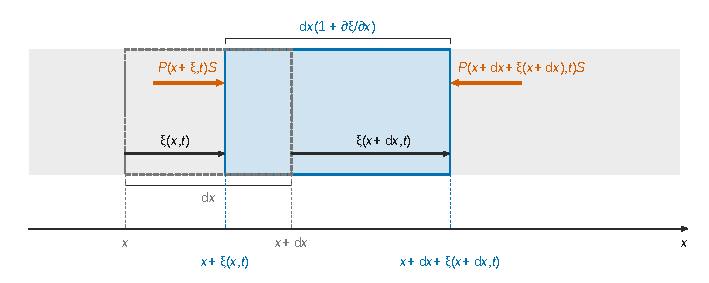
\includegraphics{figures/q19-q21-tranche-fluide.pdf}
\caption*{Figure 2 --- Tranche de fluide au repos et en mouvement, longueur dx(1 +
∂ξ/∂x) et forces de pression sur ses deux faces}
\end{figure}

À l'instant \(t\), la tranche est comprise entre \(x+\xi(x,t)\) et \(x+\mathrm dx+\xi(x+\mathrm dx,t)\). Sa longueur est
\equationajustee{\mathrm dx+\xi(x+\mathrm dx,t)-\xi(x,t)=\mathrm dx\left(1+\frac{\partial\xi}{\partial x}\right)\ \text{au premier ordre en}\ \mathrm dx ,}
et la section \(S\) est inchangée :
\equationajustee{\boxed{\mathrm d\tau\simeq S\,\mathrm dx\left(1+\frac{\partial\xi}{\partial x}\right)}}

\hypertarget{q20}{%
\subsection{Q20}\label{q20}}

La tranche est un système fermé : \(\mu_0S\,\mathrm dx=(\mu_0+\mu_1)\,S\,\mathrm dx\left(1+\dfrac{\partial\xi}{\partial x}\right)\), soit
\equationajustee{0=\mu_1+\mu_0\frac{\partial\xi}{\partial x}+\mu_1\frac{\partial\xi}{\partial x} .}
Le dernier terme est d'ordre 2, négligé :
\equationajustee{\boxed{\mu_1(x,t)\simeq-\mu_0\frac{\partial\xi}{\partial x}}\qquad(1)}

\hypertarget{q21}{%
\subsection{Q21}\label{q21}}

Système : la tranche, de masse \(\mu_0S\,\mathrm dx\), dans le référentiel terrestre galiléen ; accélération \(\partial^2\xi/\partial t^2\). Forces : pressions sur les deux faces (poids négligé) :
\equationajustee{\mu_0S\,\mathrm dx\,\frac{\partial^2\xi}{\partial t^2}=S\left[P(x+\xi,t)-P(x+\mathrm dx+\xi(x+\mathrm dx),t)\right]\simeq-S\,\frac{\partial P}{\partial x}\,\mathrm dx .}
\(P_0\) étant uniforme, \(\partial P/\partial x=\partial p_1/\partial x\), déjà d'ordre 1 ; l'évaluer en \(x+\xi\) au lieu de \(x\) ne change que des termes d'ordre 2 :
\equationajustee{\boxed{\mu_0\frac{\partial^2\xi}{\partial t^2}\simeq-\frac{\partial p_1}{\partial x}}\qquad(2)}

\hypertarget{q22}{%
\subsection{Q22}\label{q22}}

\begin{enumerate}
\def\labelenumi{(\arabic{enumi})}
\tightlist
\item
  et (3) donnent \(\dfrac{\partial\xi}{\partial x}=-\chi_sp_1\). En dérivant (2) par rapport à \(x\) (théorème de Schwarz) :
  \equationajustee{\mu_0\frac{\partial^2}{\partial t^2}\left(\frac{\partial\xi}{\partial x}\right)=-\frac{\partial^2p_1}{\partial x^2}}
  On remplace \(\partial\xi/\partial x\) par \(-\chi_sp_1\) :
  \equationajustee{-\mu_0\chi_s\frac{\partial^2p_1}{\partial t^2}=-\frac{\partial^2p_1}{\partial x^2}}
  \equationajustee{\boxed{\frac{\partial^2p_1}{\partial x^2}-\frac1{c^2}\frac{\partial^2p_1}{\partial t^2}=0}}
  avec
  \equationajustee{\boxed{c=\frac1{\sqrt{\mu_0\chi_s}}}}
\end{enumerate}

\hypertarget{q23}{%
\subsection{Q23}\label{q23}}

C'est l'\textbf{équation de d'Alembert} (équation d'onde à une dimension).

D'après (3), \(\chi_s=\mu_1/(\mu_0p_1)\) est l'inverse d'une pression : \([\chi_s]=\mathrm{Pa^{-1}}=\mathrm{kg^{-1}\cdot m\cdot s^2}\). Alors \([\mu_0\chi_s]=\mathrm{kg\cdot m^{-3}}\times\mathrm{kg^{-1}\cdot m\cdot s^2}=\mathrm{s^2\cdot m^{-2}}\) et \(c\) s'exprime en \(\mathrm{m\cdot s^{-1}}\) : c'est une vitesse.

Dans l'air, conditions usuelles : \(\boxed{c\simeq3{,}4\cdot10^2\ \mathrm{m\cdot s^{-1}}}\). Pour \(d=34\) cm :
\equationajustee{\boxed{\Delta t_{prop}=\frac dc=\frac{0{,}34}{340}\simeq1\ \mathrm{ms}}}
\textbf{Commentaire} : ce retard est très petit devant la durée du « pop » (environ 50 ms, Q24) et devant l'échelle de la figure 8 (graduée par 50 ms) : la synchronisation entre micro et caméra n'en est pas affectée.

\hypertarget{q24}{%
\subsection{Q24}\label{q24}}

Sur la figure 8, la flèche « pop » s'étend d'environ 105 ms à 155 ms :
\equationajustee{\Delta t\simeq50\ \mathrm{ms} .}
On est certain de trouver la durée dans \([40;60]\) ms, soit \(\Delta=10\) ms :
\equationajustee{u(\Delta t)=\frac{\Delta}{\sqrt3}\simeq0{,}6\times10\ \mathrm{ms}}
Résultat :
\equationajustee{\boxed{\Delta t=50\ \mathrm{ms}}}
\equationajustee{\boxed{u(\Delta t)\simeq6\ \mathrm{ms}}}

\hypertarget{q25}{%
\subsection{Q25}\label{q25}}

\equationajustee{\begin{aligned}
\Delta f&=\frac1{\Delta t}\\
&=\frac1{5\cdot10^{-2}}
\end{aligned}}
\equationajustee{\boxed{\Delta f\simeq20\ \mathrm{Hz}}}
Quotient avec un numérateur exact :
\equationajustee{\begin{aligned}
\frac{u(\Delta f)}{\Delta f}&=\frac{u(\Delta t)}{\Delta t}\\
&=\frac6{50}\\
&=0{,}12
\end{aligned}}
d'où
\equationajustee{\boxed{u(\Delta f)\simeq2\ \mathrm{Hz}}}

\hypertarget{q26}{%
\subsection{Q26}\label{q26}}

Nyquist-Shannon : \(F_E>2f_{max}\). Le spectre est centré sur \(f_0=1\) kHz, de largeur \(\Delta f\simeq20\) Hz, donc \(f_{max}\simeq f_0+\Delta f/2\simeq1{,}01\) kHz :
\equationajustee{\boxed{F_{E,min}=2f_{max}\simeq2\ \mathrm{kHz}}}

\hypertarget{q27}{%
\subsection{Q27}\label{q27}}

\equationajustee{\begin{aligned}
N_{min}&=F_{E,min}\,T_{aq}\\
&=F_{E,min}\times2\Delta t\\
&=2\cdot10^3\times0{,}1
\end{aligned}}
\equationajustee{\boxed{N_{min}\simeq2\cdot10^2\ \text{points}}}

\hypertarget{q28}{%
\subsection{Q28}\label{q28}}

La résolution du spectre calculé est \(\delta f\simeq1/T_{aq}\) (écart entre deux fréquences successives du spectre discret). Avec \(T_{aq}=0{,}1\) s, on a \(\delta f=10\) Hz, déjà comparable à \(\Delta f\simeq20\) Hz.

Diminuer \(T_{aq}\) augmente \(\delta f\) : \textbf{la résolution spectrale se dégrade}. Le pic n'est plus décrit que par un ou deux points et sa largeur \(\Delta f\) n'est plus mesurable (le spectre affiché est élargi). Le repliement, lui, ne dépend que de \(F_E\).

Problème II --- Circulations électriques dans l'atmosphère

\hypertarget{partie-i-moduxe9lisation-du-condensateur-terrestre}{%
\section{Partie I --- Modélisation du condensateur terrestre}\label{partie-i-moduxe9lisation-du-condensateur-terrestre}}

\hypertarget{q29}{%
\subsection{Q29}\label{q29}}

\textbf{Invariances} : la distribution (deux sphères concentriques uniformément chargées) est invariante par toute rotation autour du centre \(O\) : les composantes de \(\vec E\) ne dépendent que de \(r\).

\textbf{Symétries} : tout plan contenant \(O\) et \(M\) est plan de symétrie de la distribution ; \(\vec E\), vecteur polaire, appartient à tous ces plans, donc à leur intersection, la droite \((OM)\) :
\equationajustee{\boxed{\vec E=E(r)\,\vec e_r}}
\textbf{Signe} : le champ va des charges positives (ionosphère, \(+Q\)) vers les charges négatives (Terre, \(-Q\)), donc vers le centre : \(\boxed{E(r)<0}\).

\hypertarget{q30}{%
\subsection{Q30}\label{q30}}

\begin{figure}[H]
\centering
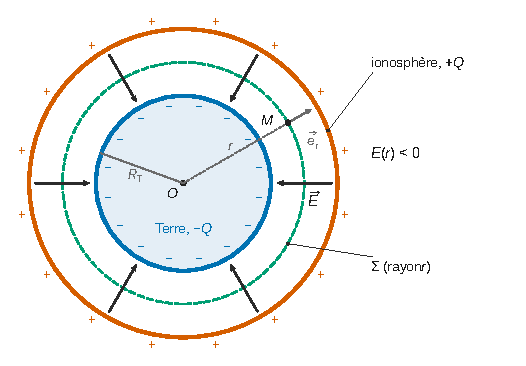
\includegraphics{figures/q29-q30-surface-gauss.pdf}
\caption*{Figure 3 --- Coupe du condensateur terrestre, champ dirigé vers la Terre
et sphère de Gauss de rayon r}
\end{figure}

Surface de Gauss : sphère \(\Sigma\) de centre \(O\) et de rayon \(r\in[R_T,R_T+h]\), orientée vers l'extérieur. D'après Q29, \(\vec E\) y est normal et de valeur uniforme : flux \(E(r)\,4\pi r^2\). La charge intérieure est celle de la Terre, \(-Q\) :
\equationajustee{E(r)\,4\pi r^2=-\frac Q{\varepsilon_0}}
d'où
\equationajustee{\boxed{E(r)=-\frac Q{4\pi\varepsilon_0r^2}}}

\hypertarget{q31}{%
\subsection{Q31}\label{q31}}

À l'altitude \(z\), \(r=R_T+z\) :
\equationajustee{-E=\frac Q{4\pi\varepsilon_0R_T^2}\left(1+\frac z{R_T}\right)^{-2}}
On note \(-E_0=Q/(4\pi\varepsilon_0R_T^2)\) la valeur au sol. En logarithme décimal, puis au premier ordre en \(z/R_T\) :
\equationajustee{\begin{aligned}
\log(-E)&=\log(-E_0)-\frac2{\ln10}\ln\left(1+\frac z{R_T}\right)\\
&\simeq\log(-E_0)-\frac2{\ln10}\,\frac z{R_T}
\end{aligned}}
Donc
\equationajustee{\boxed{z\simeq\frac{R_T\ln10}2\left[\log(-E_0)-\log(-E)\right]}}
Au premier ordre, \(z\) est une \textbf{fonction affine décroissante de \(\log(-E)\)} : \(|E|\) diminue quand l'altitude augmente, et la courbe \(z(\log(-E))\) est une droite dans le repère semi-logarithmique.

C'est l'allure globale de la figure 11a (de \(-E\simeq40\) V/m vers 1,5 km à \(-E\simeq5\) V/m vers 10 km, décroissance monotone à peu près rectiligne en semi-log) : le modèle est \textbf{globalement compatible}.

En revanche, la pente prédite (\(R_T\ln10/2\simeq7\cdot10^3\) km par décade) est bien plus grande que la pente observée (environ 10 km par décade) : la géométrie sphérique seule n'explique pas l'amplitude de la décroissance (l'atmosphère est conductrice, partie II).

\hypertarget{q32}{%
\subsection{Q32}\label{q32}}

Zone 1 de la figure 11b : \(-E\) passe de 0,2 à 0,13 kV/m environ, soit avec un chiffre significatif
\equationajustee{\boxed{-E\simeq0{,}2\ \mathrm{kV\cdot m^{-1}}=2\cdot10^2\ \mathrm{V\cdot m^{-1}}}}
Q30 en \(r=R_T\) :
\equationajustee{\begin{aligned}
Q&=4\pi\varepsilon_0R_T^2|E|\\
&=\frac{(6\cdot10^6)^2\times2\cdot10^2}{9\cdot10^9}\\
&=\frac{7{,}2\cdot10^{15}}{9\cdot10^9}
\end{aligned}}
\equationajustee{\boxed{Q\simeq8\cdot10^5\ \mathrm C}}
La Terre porte donc la charge \(-Q\simeq-8\cdot10^5\) C.

\hypertarget{q33}{%
\subsection{Q33}\label{q33}}

L'ordonnée de la figure 11b est \(-E\). Par temps calme, \(-E>0\), donc \(E<0\) : le champ est dirigé vers le sol (\(-\vec e_r\)).

La courbe décroît, s'annule vers 3 à 4 min (zone 2, temps orageux), puis reste négative pendant l'orage (\(-E\) descend jusqu'à \(-2{,}5\) kV/m). Alors \(E>0\) : le champ est dirigé vers le haut.

\textbf{Le champ électrique change de sens vers \(t\simeq3\) à \(4\) min, au passage de \(-E\) par zéro, avant le début de l'orage proprement dit.}

\hypertarget{partie-ii-courant-ionique-atmosphuxe9rique-par-beau-temps}{%
\section{Partie II --- Courant ionique atmosphérique par beau temps}\label{partie-ii-courant-ionique-atmosphuxe9rique-par-beau-temps}}

\hypertarget{q34}{%
\subsection{Q34}\label{q34}}

\([\lambda]=[F]/[v]=\mathrm{kg\cdot m\cdot s^{-2}}/(\mathrm{m\cdot s^{-1}})\) :
\equationajustee{\boxed{\lambda\ \text{en}\ \mathrm{kg\cdot s^{-1}}}}

\hypertarget{q35}{%
\subsection{Q35}\label{q35}}

Système : l'ion (\(m\), \(+e\)) ; référentiel terrestre galiléen ; forces : \(e\vec E\) et \(-\lambda\vec v\) (poids et force magnétique négligés). Principe fondamental de la dynamique :
\equationajustee{\boxed{m\frac{\mathrm d\vec v}{\mathrm dt}+\lambda\vec v=e\vec E}}

\hypertarget{q36}{%
\subsection{Q36}\label{q36}}

Équation linéaire du premier ordre de constante de temps \(m/\lambda\) ; le régime transitoire s'amortit et, en régime permanent, \(\mathrm d\vec v/\mathrm dt=\vec0\) :
\equationajustee{\boxed{\vec v_\ell=\frac e\lambda\,\vec E}}

\hypertarget{q37}{%
\subsection{Q37}\label{q37}}

\equationajustee{\boxed{\vec j_c=n\,e\,\vec v_\ell=\frac{ne^2}\lambda\,\vec E}}

\hypertarget{q38}{%
\subsection{Q38}\label{q38}}

Pour un anion (charge \(-e\), même \(\lambda\)) : \(\vec v_{\ell,a}=-\dfrac e\lambda\vec E\) et \(\vec j_a=n(-e)\vec v_{\ell,a}=\dfrac{ne^2}\lambda\vec E\). Les deux contributions sont de même sens :
\equationajustee{\boxed{\vec j=\vec j_a+\vec j_c=2n\frac{e^2}\lambda\,\vec E}}
C'est une loi d'Ohm locale ; comme \(E(z)<0\), le courant est descendant.

\hypertarget{q39}{%
\subsection{Q39}\label{q39}}

Chaque famille d'ions obéit à la loi d'Ohm locale : \(\vec j_a=\gamma_a\vec E\) et \(\vec j_c=\gamma_c\vec E\). On a donc calculé, \textbf{à chaque altitude}, le produit de la conductivité mesurée par la valeur du champ mesurée à la même altitude (figure 12a) :
\equationajustee{\boxed{j_a(z)=\gamma_a(z)\,|E(z)|}}
\equationajustee{\boxed{j_c(z)=\gamma_c(z)\,|E(z)|}}
Exemple : vers 3 km, \(\gamma_a\simeq8\cdot10^{-14}\) S/m et \(|E|\simeq25\) V/m donnent \(j_a\simeq2\cdot10^{-12}\) A/m² ; vers 10 km, \(4\cdot10^{-13}\) S/m et 5 V/m donnent la même valeur.

\hypertarget{q40}{%
\subsection{Q40}\label{q40}}

La figure 12b donne \(j_a\simeq j_c\simeq2\cdot10^{-12}\) A·m⁻² à toutes les altitudes (densité moyenne). La densité totale est leur somme :
\equationajustee{\boxed{j_{mes}=j_a+j_c\simeq4\cdot10^{-12}\ \mathrm{A\cdot m^{-2}}}}
\textbf{La valeur annoncée est compatible avec la mesure.}

\hypertarget{partie-iii-duxe9charge-du-condensateur-terrestre}{%
\section{Partie III --- Décharge du condensateur terrestre}\label{partie-iii-duxe9charge-du-condensateur-terrestre}}

\hypertarget{q41}{%
\subsection{Q41}\label{q41}}

\(\vec j\) uniforme et normal à la surface : \(I=jS_T=4\cdot10^{-12}\times5\cdot10^{14}\)
\equationajustee{\boxed{I\simeq2\cdot10^3\ \mathrm A}}

\hypertarget{q42}{%
\subsection{Q42}\label{q42}}

Par définition, \(I=\left|\dfrac{\mathrm dq}{\mathrm dt}\right|\). En supposant \(I\) constant, la charge \(Q\) est neutralisée au bout de \(\tau\) tel que \(Q=I\tau\) :
\equationajustee{\boxed{\tau=\frac QI}}

\hypertarget{q43}{%
\subsection{Q43}\label{q43}}

Avec Q32 et Q41, \(\tau=8\cdot10^5/2\cdot10^3=4\cdot10^2\) s, en accord avec la valeur annoncée. Sept minutes : le condensateur terrestre serait déchargé en quelques minutes. Or le champ de beau temps est observé en permanence et la différence de potentiel reste constante. \textbf{Le modèle d'un condensateur isolé qui se décharge est incomplet : il faut un mécanisme de recharge permanent (un générateur)}, que les parties IV et V identifient aux orages.

\hypertarget{partie-iv-recharge-du-condensateur-terrestre}{%
\section{Partie IV --- Recharge du condensateur terrestre}\label{partie-iv-recharge-du-condensateur-terrestre}}

\hypertarget{q44}{%
\subsection{Q44}\label{q44}}

\textbf{Invariances} : le fil infini d'axe \(Oz\) est invariant par translation selon \(z\) et par rotation autour de \(Oz\) : \(\vec B(M)=\vec B(d,t)\) (ARQS : le temps n'est qu'un paramètre).

\textbf{Symétries} : le plan \((M,\vec e_r,\vec e_z)\) contient le fil ; c'est un plan de symétrie de la distribution de courant. \(\vec B\), pseudo-vecteur, est orthogonal à ce plan :
\equationajustee{\boxed{\vec B=B(d,t)\,\vec e_\theta}}

\hypertarget{q45}{%
\subsection{Q45}\label{q45}}

Contour \(\mathcal C\) : cercle de rayon \(d\) centré sur le fil, dans un plan perpendiculaire à \(Oz\), orienté selon \(\vec e_\theta\) (normale \(+\vec e_z\), sens du courant). \(\vec B\) y est tangent et de norme uniforme. Théorème d'Ampère (valable dans l'ARQS) :
\equationajustee{B(d,t)\,2\pi d=\mu_0\,i(t)}
d'où
\equationajustee{\boxed{\vec B=\frac{\mu_0\,i(t)}{2\pi d}\,\vec e_\theta}}

\hypertarget{q46}{%
\subsection{Q46}\label{q46}}

Champ uniforme sur la bobine : flux à travers les \(N\) spires
\equationajustee{\Phi=N\,\vec B\cdot\vec S_1=NS_1\frac{\mu_0\,i(t)}{2\pi d}\cos\alpha .}
Seul \(i\) dépend du temps ; loi de Faraday :
\equationajustee{\begin{aligned}
e_1&=-\frac{\mathrm d\Phi}{\mathrm dt}\\
&=-NS_1\frac{\mu_0}{2\pi d}\frac{\mathrm di}{\mathrm dt}\cos\alpha
\end{aligned}}
Par identification avec l'expression de l'énoncé :
\equationajustee{\boxed{f(\alpha)=\cos\alpha}}

\hypertarget{q47}{%
\subsection{Q47}\label{q47}}

Basse fréquence : le condensateur est un interrupteur ouvert ; haute fréquence : un fil.

\begin{itemize}
\tightlist
\item
  Filtre A (sortie aux bornes de \(C\)) : en BF, aucun courant, \(v_s=v_e\) ; en HF, \(C\) court-circuite la sortie, \(v_s=0\). Passe-bas, gain 1 puis 0.
\item
  Filtre B (sortie aux bornes de \(R\)) : en BF, \(C\) bloque le courant, \(v_s=0\) ; en HF, \(v_s=v_e\). Passe-haut.
\end{itemize}

\begin{figure}[H]
\centering
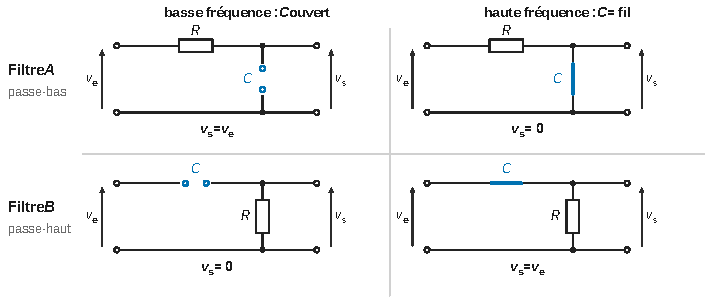
\includegraphics{figures/q47-filtres-bf-hf.pdf}
\caption*{Figure 4 --- Filtres A et B en basse fréquence (C ouvert) et en haute
fréquence (C remplacé par un fil)}
\end{figure}

Or \(|\underline H_1|\to1\) en BF et \(\to0\) en HF ; \(|\underline H_2|\to0\) en BF et \(\to1\) en HF :
\equationajustee{\boxed{\underline H_1\leftrightarrow\text{filtre A},\qquad\underline H_2\leftrightarrow\text{filtre B}}}
(Le diviseur de tension le confirme : \(\underline H_A=\dfrac{1/(jC\omega)}{R+1/(jC\omega)}=\dfrac1{1+jRC\omega}\).)

\hypertarget{q48}{%
\subsection{Q48}\label{q48}}

Un intégrateur a une fonction de transfert de la forme \(\dfrac1{j\omega\tau_0}\). Pour \(RC\omega\gg1\) :
\equationajustee{\underline H_1\simeq\frac1{jRC\omega}}
En temporel, diviser par \(j\omega\) revient à intégrer :
\equationajustee{v_s\simeq\frac1{RC}\int v_e\,\mathrm dt .}
\equationajustee{\boxed{\text{Le filtre A est \text{intégrateur} pour}\ \omega\gg\frac1{RC},\ \text{soit}\ f\gg\frac1{2\pi RC}}}
Appliqué à \(e_1\propto\mathrm di/\mathrm dt\), il restitue un signal proportionnel à \(i(t)\). (Le filtre B serait dérivateur en basse fréquence.)

\hypertarget{partie-v-intensituxe9-duxe9placuxe9e-par-les-orages}{%
\section{Partie V --- Intensité déplacée par les orages}\label{partie-v-intensituxe9-duxe9placuxe9e-par-les-orages}}

\hypertarget{q49}{%
\subsection{Q49}\label{q49}}

Le rapport \(e_2/e_1\) élimine \(N\), \(S_1\), \(d\) et \(\mathrm di/\mathrm dt\).

Sur la figure 15b (1 V/div), les deux tensions ont la même forme. Au sommet, \(e_1\simeq2{,}4\) V et \(e_2\simeq2{,}2\) V :
\equationajustee{\tan\alpha=\frac{e_2}{e_1}\simeq0{,}9}
\equationajustee{\boxed{\alpha\simeq42^\circ\ \text{(environ}\ 45^\circ)}}
\textbf{Le champ magnétique est horizontal, dans le plan des deux vecteurs surface, et fait un angle d'environ 42° avec \(\vec S_1\)}, à peu près selon la bissectrice de \(\vec S_1\) et \(\vec S_2\).

Comme \(\vec B\) est porté par \(\vec e_\theta\), l'éclair se trouve dans la direction perpendiculaire à \(\vec B\) (selon \(\vec e_r\)).

\hypertarget{q50}{%
\subsection{Q50}\label{q50}}

D'après Q46, \(|e_1|=NS_1\dfrac{\mu_0}{2\pi}\cos\alpha\cdot\dfrac1d\left|\dfrac{\mathrm di}{\mathrm dt}\right|\). La distance n'apparaît que dans le rapport \(\dfrac1d\left|\dfrac{\mathrm di}{\mathrm dt}\right|\), et le courant de l'éclair est inconnu : un éclair faible et proche donne le même signal qu'un éclair intense et lointain. Un détecteur fournit la direction de l'éclair (Q49), \textbf{pas sa distance}.

\hypertarget{q51}{%
\subsection{Q51}\label{q51}}

Chaque détecteur donne une droite de visée : la droite passant par le détecteur, perpendiculaire à \(\vec B\) mesuré. Deux droites non parallèles se coupent en un point unique :
\equationajustee{\boxed{\text{2 \text{détecteurs} au minimum}}}

\begin{figure}[H]
\centering
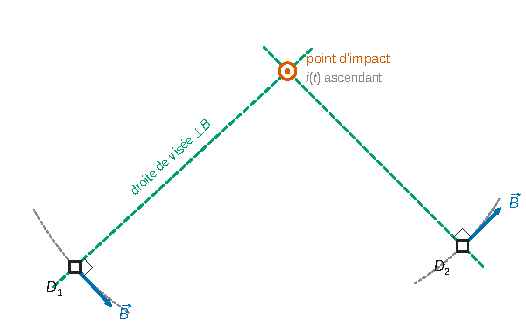
\includegraphics{figures/q51-localisation-deux-detecteurs.pdf}
\caption*{Figure 5 --- Vue de haut, deux droites de visée perpendiculaires au
champ mesuré se coupent au point d'impact}
\end{figure}

La construction échoue si l'éclair est aligné avec \(D_1\) et \(D_2\) (droites confondues) ; un troisième détecteur lève ce cas et améliore la précision.

\hypertarget{q52}{%
\subsection{Q52}\label{q52}}

Figure 16 : environ 1,7 kA (décembre-février), 2,2 kA (mars-mai), 2,4 kA (juin-août), 2,0 kA (septembre-novembre). Moyenne annuelle :
\equationajustee{\boxed{I_{\text{orages}}\simeq2\ \mathrm{kA}=2\cdot10^3\ \mathrm A}}

\hypertarget{q53}{%
\subsection{Q53}\label{q53}}

\(I_{\text{\text{décharge}}}=jS_T\simeq2\cdot10^3\) A (Q41) et \(I_{\text{orages}}\simeq2\cdot10^3\) A (Q52) sont égales à un chiffre significatif. Les orages font circuler les charges en sens opposé au courant de beau temps, d'où
\equationajustee{\frac{\mathrm dQ_{\text{Terre}}}{\mathrm dt}=I_{\text{orages}}-I_{\text{\text{décharge}}}\simeq0 .}
\textbf{Oui, les orages compensent la décharge naturelle du condensateur terrestre}, qui reste chargé en régime stationnaire : ils jouent le rôle du générateur qui manquait en Q43.

FIN

\end{document}
